% ==================================================
\chapter{Related Work}\label{chap:Related Work}
% ==================================================

There has been work on the quantification of academic careers, focused on a quest for a `number' that sums up an academic's scholarship. The most well-known outcome of this line of research is the {\it h}-index, proposed by Hirsch \cite{Hirsch:2005}. A scholar has an index of {\it h} if s/he has published {\it h} papers each of which has been cited in other papers at least {\it h} times (Figure \ref{fig-hindex}).

\begin{figure*}
    \centering
    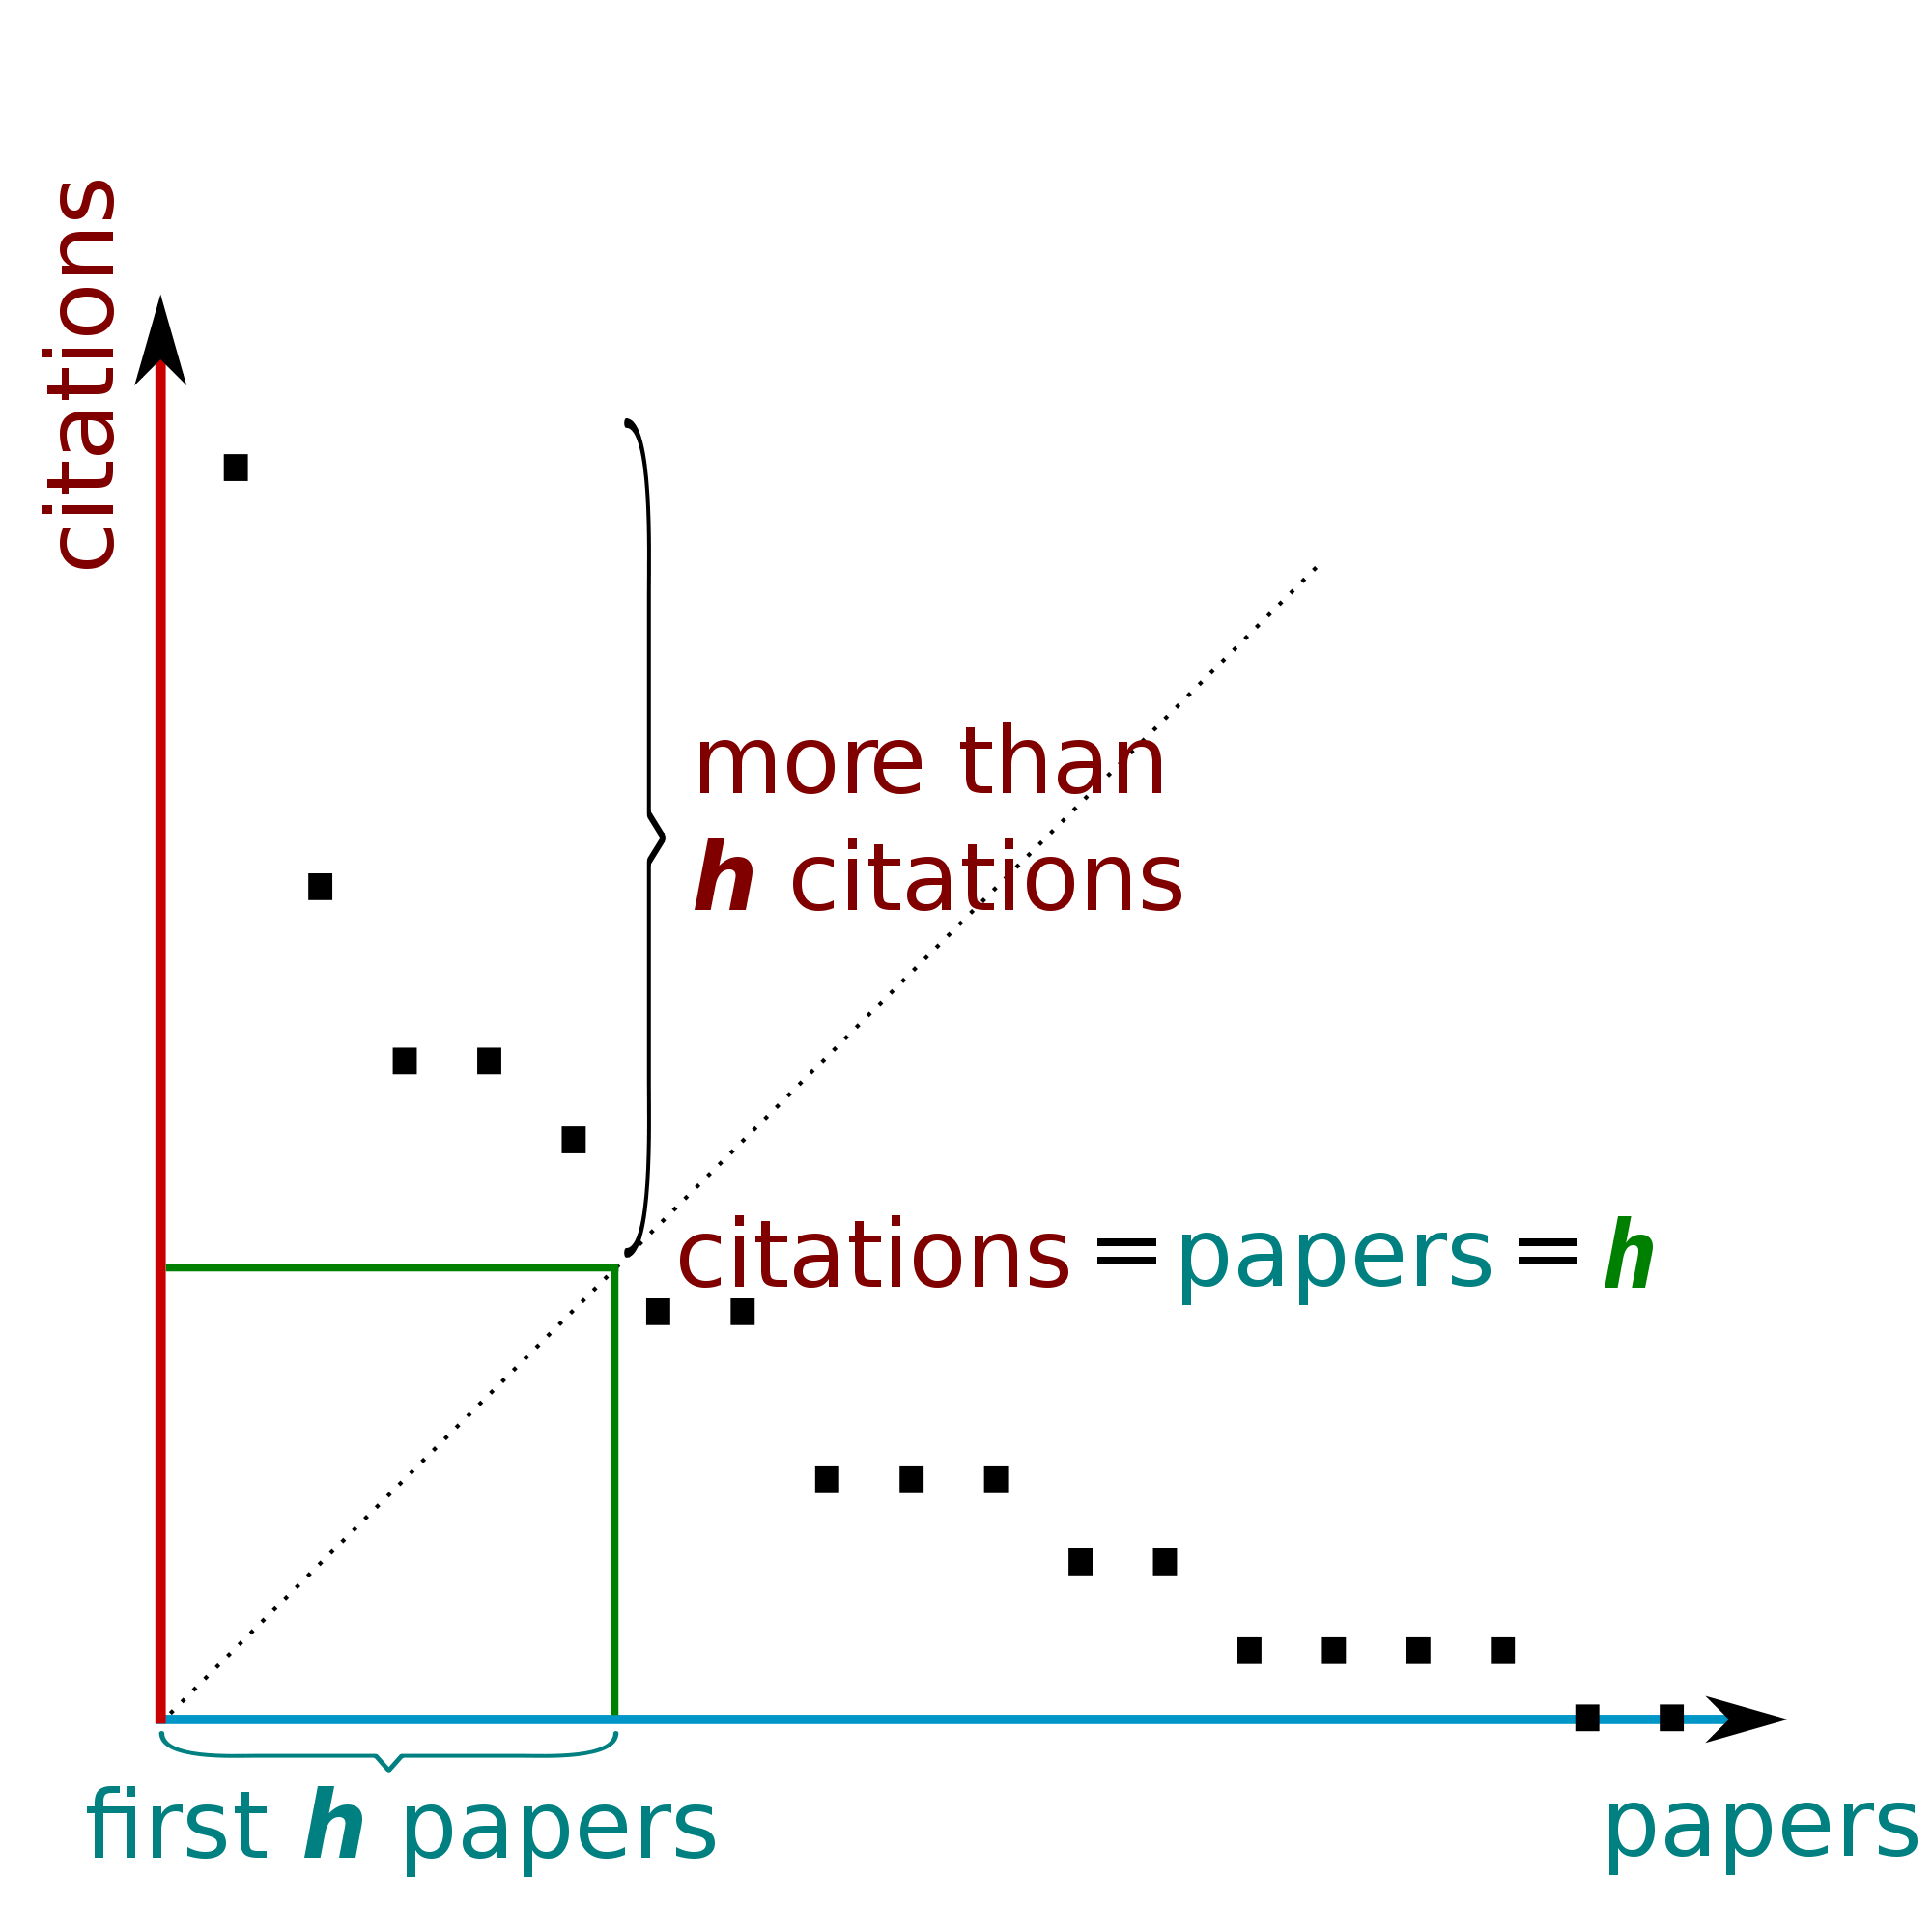
\includegraphics[width=.3\textwidth]{figures/H-index.png}
    \caption{h-index from a plot of decreasing citations for numbered papers.}~\label{fig-hindex}
\end{figure*}


The {\it h}-index depends on both the number of publications and the number of citations. Hirsch demonstrated that {\it h} can predict honors, such as the National Academy membership and the Nobel prize. He also suggested that it could predict advancement to tenure, although with some uncertainty.
Despite its value, the {\it h}-index has weaknesses and when used, context should be carefully taken into account; such context includes the academic field and the academic age of the candidate \cite{Bornmann2}.

With the advent of Google Scholar \cite{Googl82:online}, information about a researcher's publication record and her/his {\it h}-index has become easily accessible. Then, with the ease of access of the internet, this information has become ubiquitous.

In this dissertation, I introduce data visualization methods that complement publication information contained in a standard CV and summarized by the {\it h}-index. The tool produces a temporal visualization that connects the {\it h}-index with the paper citations and the journal impact factors along with funding data.

There have been other efforts in visualizing patterns of scientific production and impact \cite{Katy:2010, Chen:2001, Leydesdorff:2007}. Recently, a mobile app (DBIScholar) has also appeared that interfaces information from Google Scholar \cite{sabrina741}. A social tool named Scholarometer has been developed to facilitate citation analysis and to evaluate the impact of authors \cite{Kaur:2014}. This tool helps to visualize author and discipline networks. There is another tool called SciVal Expert, which visualizes the collaboration and research output of institutions \cite{Vardell:2011}. This tool uses data from Elsevier's Scopus, the largest abstract and citation database of peer-reviewed literature \cite{Scopu91:online}. However, these tools do not provide a visual picture of a single scholar's achievements.

The method and application differ from the prior art. At a glance, Scholar Plot helps the reviewer determine where the researcher's impact (if any) arises from.% : citations in articles published in low impact journals or citations in articles published in high impact journals.

Students need more information to decide about their college. Nowadays, a university has a ranking as well as each department with each college in that university. So students need publicly accessible information which is cheap and get a summary of various measures being used to evaluate faculty. Rankings are used to make choices to avoid risks of joining lower ranking colleges \cite{mcdonough1998college}.

The goal of research is to articulate a clear, comprehensive, and measurable performance evaluation scheme for academics. This scheme should reveal causal relationships among the merit criteria. This research provides a summary interface to facilitate executive decisions. The tool produces a temporal visualization that connects the {\it h}-index with the paper citations, and the journal impact factors along with funding data. Scholar Plot helps the reviewer determine at a glance where the researcher's impact (if any) arises from.


Here, I introduce a data visualization tool that complements the US News Rankings and the publication information contained in a standard CV. Visualization facilitates access to data and supports actionable insights \cite{Yi:2008:UCI}. It also helps to bring out patterns and pattern violations in the underlying data.
%The tool produces a temporal visualization that connects the {\it h}-index with the paper citations and the impact factors along with the funding data. Our method and application differ from the prior art. Scholar Plot helps the reviewer determine at a glance from where the researcher's impact (if any) arises from. It also gives a hierarchical view of accomplishments from a single author to the department to the entire college.